
Una vegada havia implementat la distancia de Férchet per poder avaluar el rendiment dels models, havia arribat a una clara conclusió:

Els models que tenen implementada la funció no-lienal són més eficients. 

No és exactament així perquè s'ha de tenir en compte el temps que triguen en optimitzar-se, no obstant, trec aquesta conclusió pel fet que els models sense la funció no arriben a estabilitzar-se. Fins el que puc veure, es queden oscil·lant entre 'aquestes imatges són idèntiques' i 'encara queda per optimitzar'. En una iteració les imatges són pràcticament iguals i al cap de 20 iteracions es pot diferenciar clarament entre una imatge falsa i una generada. 

Aquest problema no es causat pel discriminador, és el generador el que es queda oscil·lant. No sé molt bé la causa d'aquesta oscil·lació, però està clar que la funció no-lineal té un impacte. Tot i que hi han excepcions, a vegades els models sense la funció no experimenten aquesta oscil·lació. Però cal remarcar que les vegades que passa són notablement més altes que les que no passa. Com es pot veure amb les dades de la taula \ref{tab:oscilations} 

\begin{table}[]
	\resizebox{\textwidth}{!}{%
		\begin{tabular}{c|c|c}
			\hline
			& Presenta oscil·lació & No Presenta oscil·lació \\
			\hline
			Amb Funció No-Lineal & 0 & 6 \\
			\hline
			Sense Funció No-Lineal& 5 & 1 \\
			\hline
		\end{tabular}
	}
	\caption{Les dades provenen d'un total de 6 model, 3 d'ells amb un total de $700$ epoch i els altres 5 amb un total de $550$. El nombre d'iteraccions no hauria d'afectar de cada manera les dades. Degut si hi ha una oscil·lació, es pot veure clarament a partir de les $400$ iteracions. Amb les dades es pot veure que és més probable que un model sense la funció lienal presenti una oscil·lació. Cal notar que cap model amb la funció ha tingut una oscil·lació. Les gràfiques que corresponen a cada model es poden veure en la figura \_.}
	\label{tab:oscilations}
\end{table}

\begin{figure}
	\begin{subfigure}[b]{.32\linewidth}
		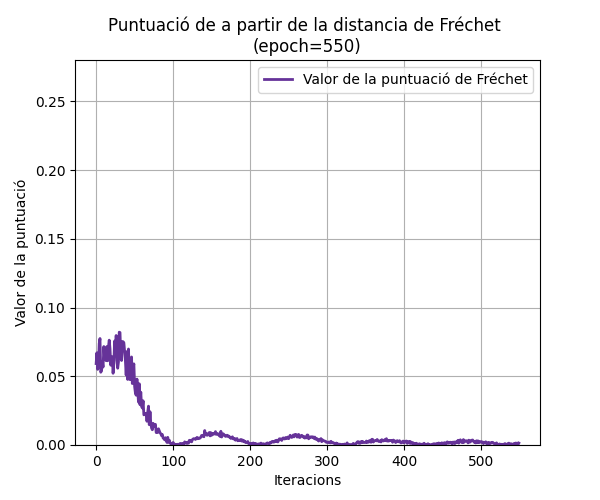
\includegraphics[width=\linewidth]{figures/data/FD_score_1.png}
		\caption{}
	\end{subfigure}
	\begin{subfigure}[b]{.32\linewidth}
		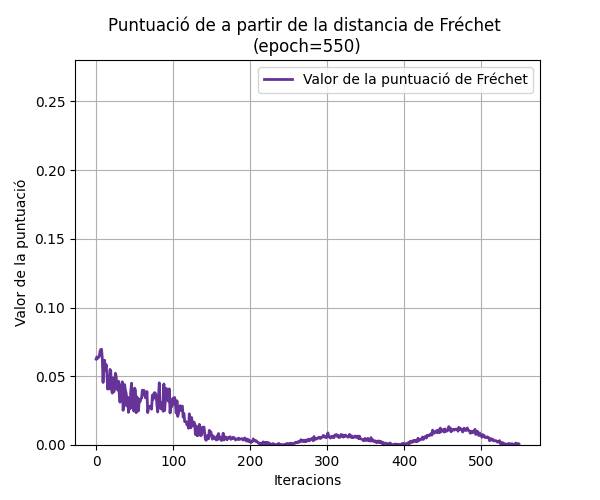
\includegraphics[width=\linewidth]{figures/data/FD_score_2.png}
		\caption{}
	\end{subfigure}
	\begin{subfigure}[b]{.32\linewidth}
		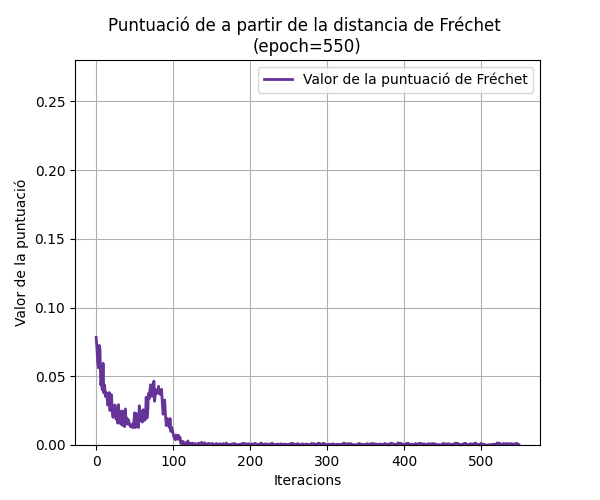
\includegraphics[width=\linewidth]{figures/data/FD_score_3.png}
		\caption{}
	\end{subfigure}
	
	\begin{subfigure}[b]{.32\linewidth}
		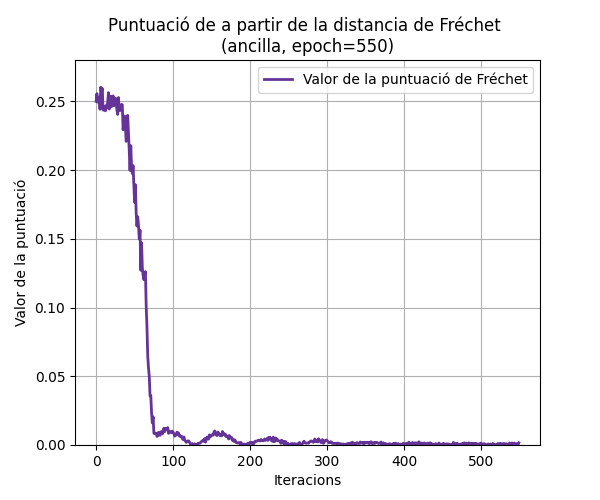
\includegraphics[width=\linewidth]{figures/data/FD_score_A1.png}
		\caption{}
	\end{subfigure}
	\begin{subfigure}[b]{.32\linewidth}
		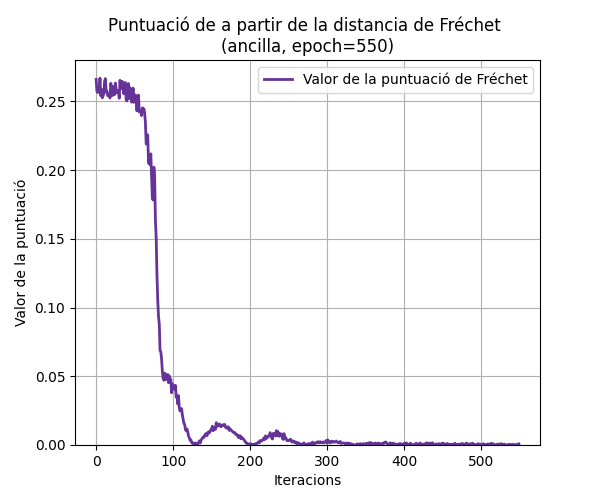
\includegraphics[width=\linewidth]{figures/data/FD_score_A2.png}
		\caption{}
	\end{subfigure}
	\begin{subfigure}[b]{.32\linewidth}
		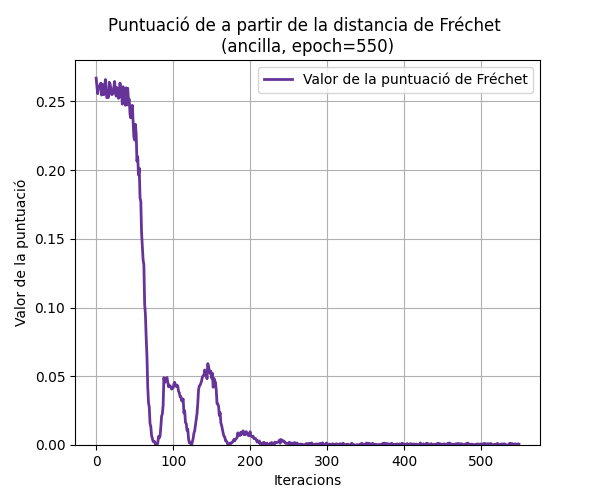
\includegraphics[width=\linewidth]{figures/data/FD_score_A3.png}
		\caption{}
	\end{subfigure}
\label{fig:550_SD_score}
\caption{Totes les gràfiques corresponen a models que s'ha executat al llarg de $550$ iteracions. \textbf{A}, \textbf{B} i \textbf{C}, corresponen a models sense la funció lineal. Es l'únic d'ells que no presenta una oscil·lació és el \textbf{C}. Les gràfiques sense la funció es poden comparar a les d'abaix, les quals representen models amb la funció. Els models han estat creats per parelles, les quals estan organitzades verticalment. Es a dir, les gràfiques \textbf{A} i \textbf{D} representen models que tenen els mateixos paràmetre inicial, que són equivalents. El mateix passa amb \textbf{B} i \textbf{E} i d'una altra banda amb \textbf{C} i \textbf{F}.}
	
\end{figure}

\begin{figure}
	\begin{subfigure}[b]{.32\linewidth}
		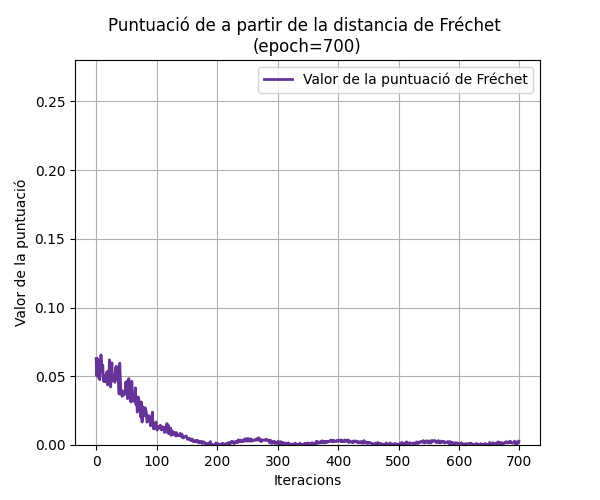
\includegraphics[width=\linewidth]{figures/data/FD_score_4.png}
		\caption{}
	\end{subfigure}
	\begin{subfigure}[b]{.32\linewidth}
		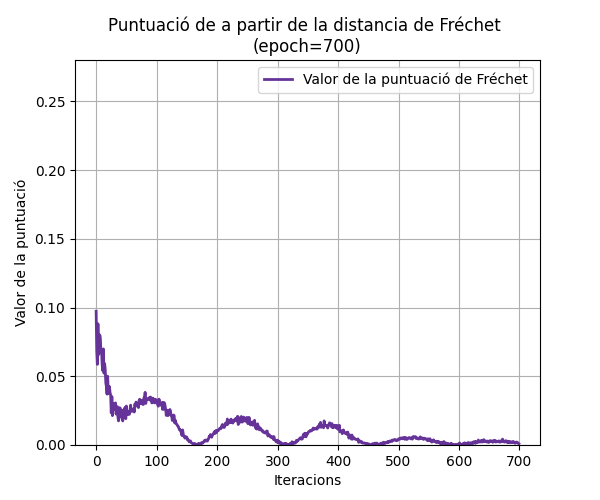
\includegraphics[width=\linewidth]{figures/data/FD_score_5.png}
		\caption{}
	\end{subfigure}
	\begin{subfigure}[b]{.32\linewidth}
		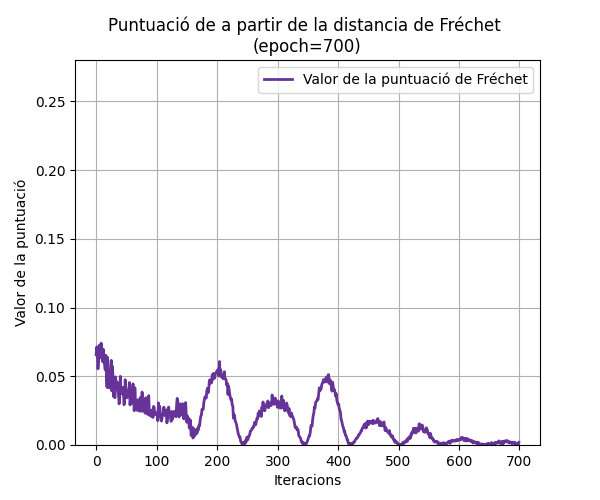
\includegraphics[width=\linewidth]{figures/data/FD_score_6.png}
		\caption{}
	\end{subfigure}
	
	\begin{subfigure}[b]{.32\linewidth}
		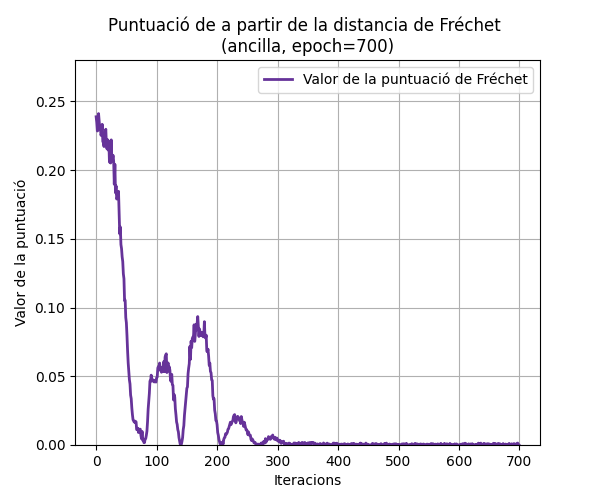
\includegraphics[width=\linewidth]{figures/data/FD_score_A4.png}
		\caption{}
	\end{subfigure}
	\begin{subfigure}[b]{.32\linewidth}
		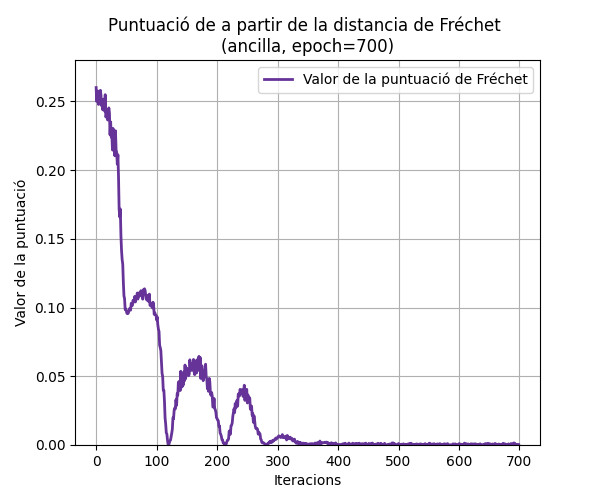
\includegraphics[width=\linewidth]{figures/data/FD_score_A5.png}
		\caption{}
	\end{subfigure}
	\begin{subfigure}[b]{.32\linewidth}
		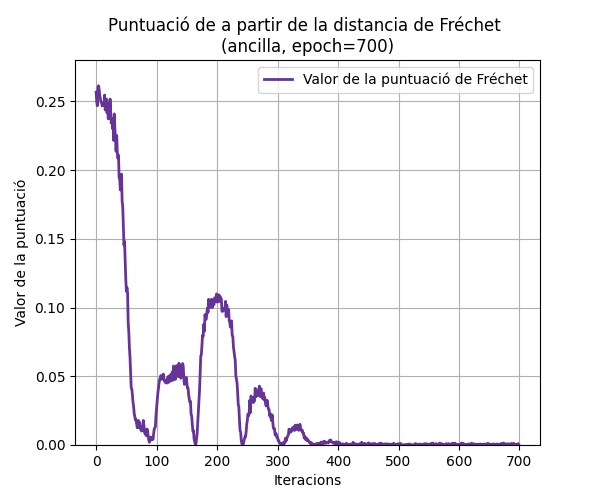
\includegraphics[width=\linewidth]{figures/data/FD_score_A6.png}
		\caption{}
	\end{subfigure}
	\label{fig:700_SD_score}
	\caption{Aquestes gràfiques corresponen a models que s'han executat al llarg de $700$ iteracions. Estan organitzades igual que les gràfiques de la figura \ref{fig:550_SD_score}. En aquests casos, com es pot observar tots els models sense la funció no-lineal presenten les oscil·lacions. No obstant en la gràfica \textbf{A}, aquesta es molt feble. Per veure com afecten les oscil·lacions es pot veure la figura, on estan representades les ultimes imatges que han generat els models que corresponen les gràfiques d'aquesta figura.}
	
\end{figure}

\begin{figure}
	\begin{subfigure}[b]{.32\linewidth}
		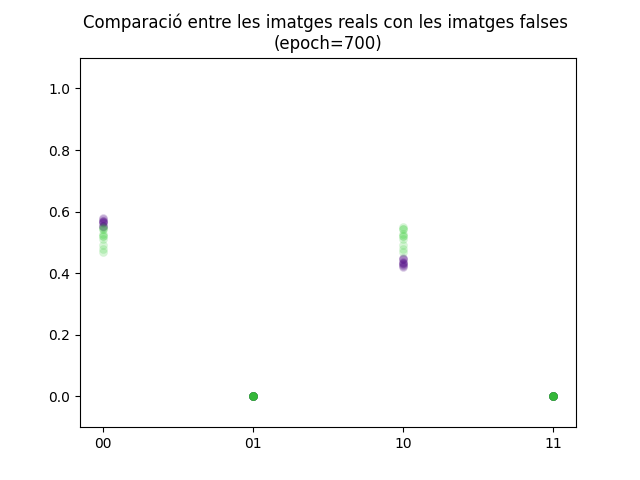
\includegraphics[width=\linewidth]{figures/data/scatter_plot_4.png}
		\caption{}
	\end{subfigure}
	\begin{subfigure}[b]{.32\linewidth}
		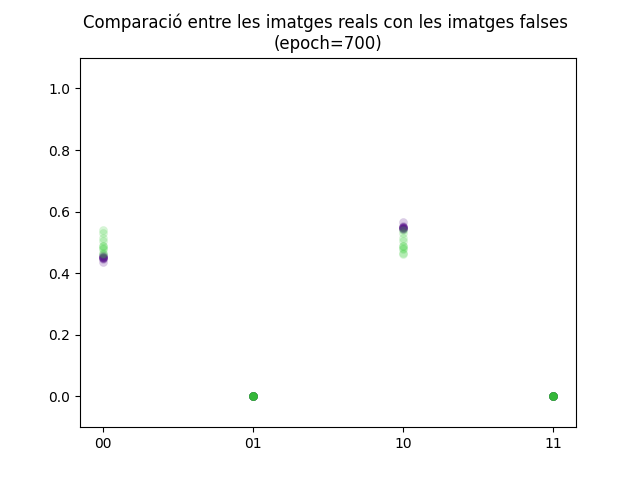
\includegraphics[width=\linewidth]{figures/data/scatter_plot_5.png}
		\caption{}
	\end{subfigure}
	\begin{subfigure}[b]{.32\linewidth}
		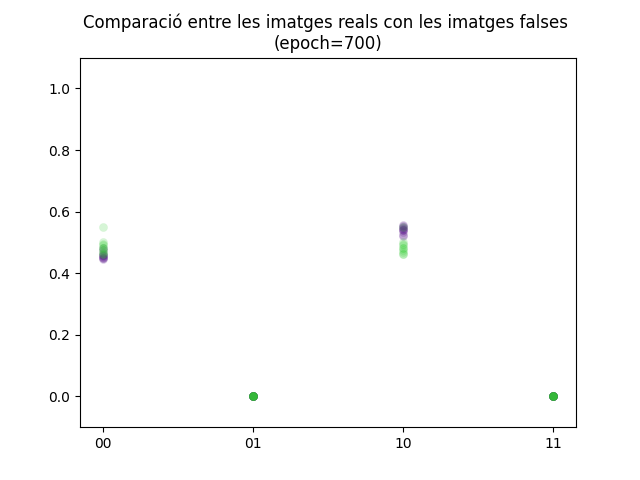
\includegraphics[width=\linewidth]{figures/data/scatter_plot_6.png}
		\caption{}
	\end{subfigure}
	
	\begin{subfigure}[b]{.32\linewidth}
		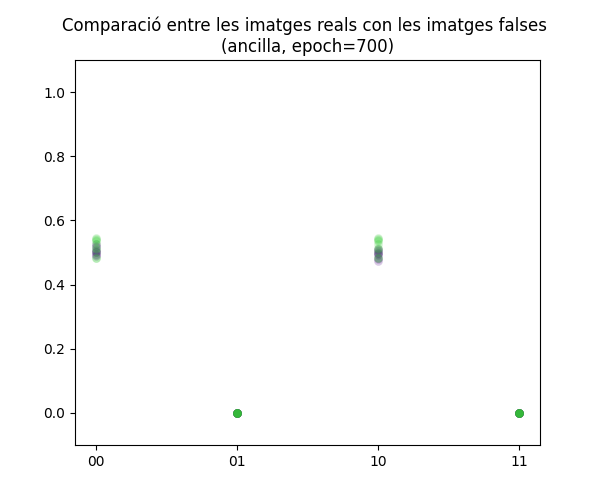
\includegraphics[width=\linewidth]{figures/data/scatter_plot_A4.png}
		\caption{}
	\end{subfigure}
	\begin{subfigure}[b]{.32\linewidth}
		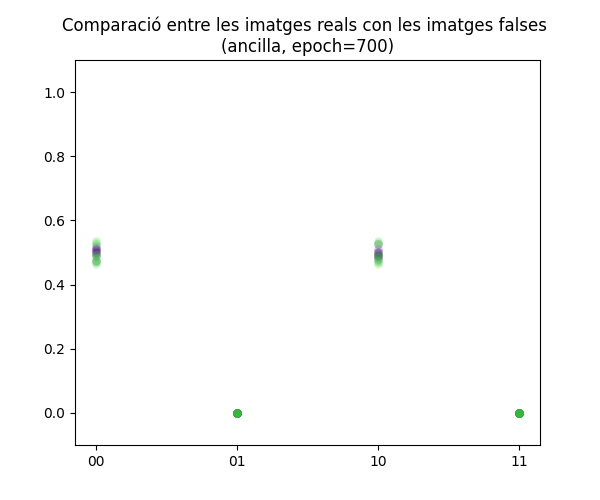
\includegraphics[width=\linewidth]{figures/data/scatter_plot_A5.png}
		\caption{}
	\end{subfigure}
	\begin{subfigure}[b]{.32\linewidth}
		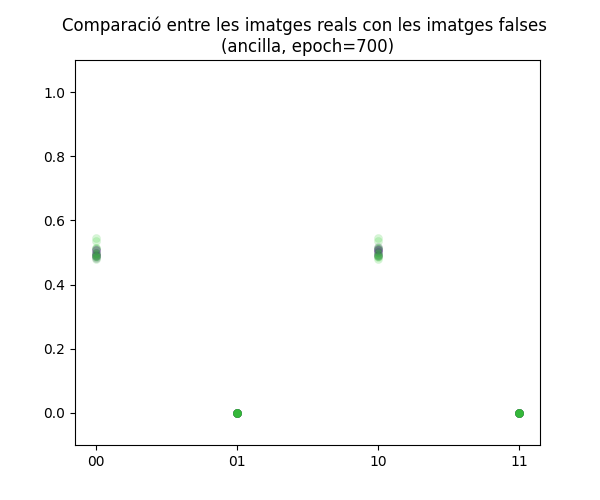
\includegraphics[width=\linewidth]{figures/data/scatter_plot_A6.png}
		\caption{}
	\end{subfigure}
	\label{fig:700_images}
	\caption{Aquestes gràfiques corresponen als mateixos models que els de la figura \ref{fig:700_SD_score}. Les posicions de les gràfiques són les mateixes, per tant si estan en la mateixa posició que les de l'altra figura, corresponen al mateix model. Les imatges generades pels models sense la funció no-lienal  (\textbf{A}, \textbf{C}, \textbf{B}) no s'asemblen a les reals. Es pot veure com els punts de les imatges generades (color violeta) no estan en els mateixos valors. Mentre que en les gràfiques \textbf{D}, \textbf{E} i \textbf{F}, si que ho estan. Els punts violetes sembla que representen la mitjana dels punts verd. També es pot observar que les imatges generades tendeixen a ser més variades que les reals.}
	
\end{figure}



